\subsection{Sonelgaz prépare le lancement d'un compteur électrique intelligent:}

Dans une déclaration à la presse en marge de l'ouverture de la 3e édition du Salon de l’électricité et des énergies renouvelables au Palais des expositions (Alger), M. Boulakhras a précisé que la Sonelgaz a fabriqué le prototype en collaboration avec l'Entreprise nationale des industries électroniques (ENIE) qui fournira au compteur intelligent la carte-mère.

Pour s'assurer de son efficacité sur le terrain, ce compteur intelligent conçu par des compétences nationales sera testé sur une période de six mois, dans deux sites au nord et au sud du pays.

Dès 2021, la Sonelgaz généralisera son utilisation au plan national, a fait savoir M. Boulakhras qui a révélé que la production des nouveaux compteurs se fera au niveau de l'Entreprise nationale des appareils de mesure et de contrôle (AMC) relevant du groupe dans la région d'El-Eulma.

A une question sur le retard du lancement de ce compteur, le PDG de la Sonelgaz a déclaré que "de nombreux pays ont opté pour la solution facile qui est l'importation du compteur intelligent, contrairement à nous qui avons opté pour une intégration nationale. Certes nous avons tardé, mais ce produit "made in algeria" est actuellement disponible".

Ce compteur intelligent est en parfaite adaptation avec le réseau local de production électrique par énergies renouvelables. Il permet d'organiser la consommation de l'énergie entre les réseau local (on-grid) et central (off-grid) de la Sonelgaz et permet de faire basculer l'excédent du réseau local au réseau central.
\\
\begin{figure}[h]
	\centering
    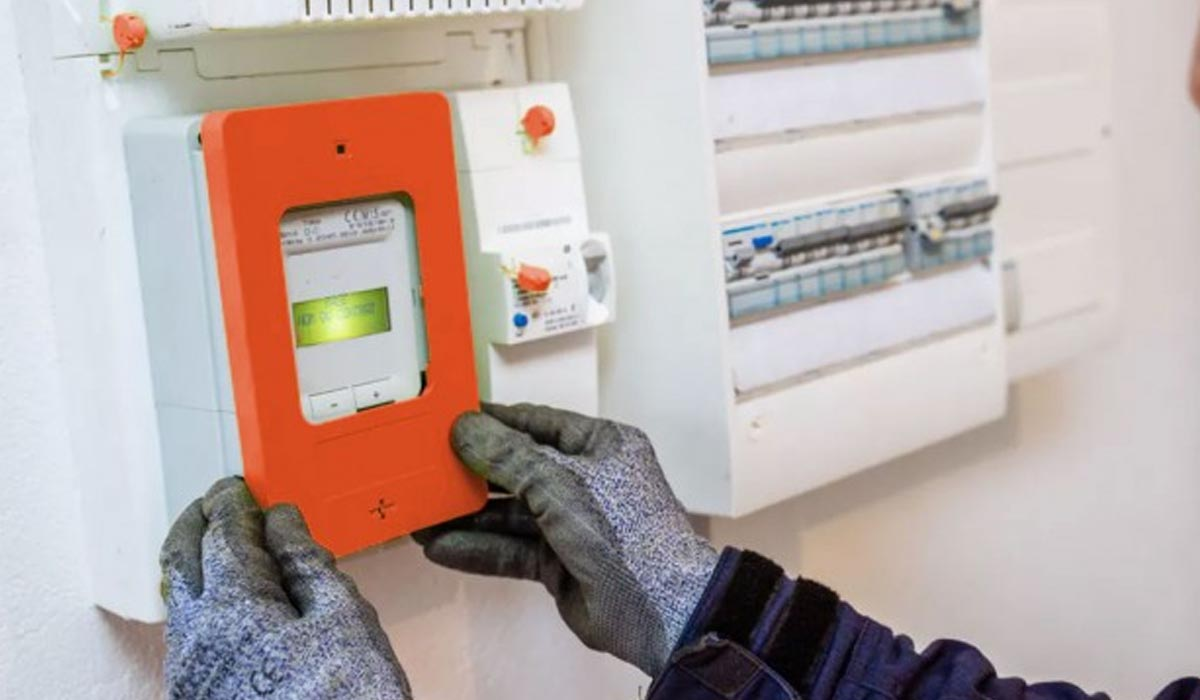
\includegraphics[scale=0.3]{img/part2/1.7}
    \caption{Compteur intelligent en Algérie}
\end{figure}